\section{AIS Tradeflows}

AIS Trade Flow systems utilize data transmitted by vessels worldwide to offer real-time and historical insights into maritime trade activities.
The objective is to establish a system that defines trade between ports based on AIS signals.
Defining port areas within AIS Trade Flow systems is a complex process that takes into account both geographical and operational considerations.
Geographically, a port area is typically defined by a specific set of coordinates that delineate the physical boundaries of the port and its surrounding waters.
This definition may encompass berths, anchorages, and sometimes even approach channels. Determining whether a ship is within a port area often involves comparing the ship's current AIS-reported coordinates with the defined boundaries of the port.
If the ship's position falls within these boundaries, it is considered to be inside the port area. However, the determination is not solely based on geographical location.
Operational factors also come into play.
For instance, a ship may be within the geographical boundaries of a port, but if it is merely passing through without stopping or engaging in port activities, it may not be considered "in port" from an operational perspective.

To address these complexities, AIS Trade Flow systems frequently employ sophisticated algorithms to accurately establish port boundaries and classify vessel behavior.
These algorithms take into account various factors such as the ship's speed, course, and historical behavior patterns.
By integrating these diverse data points, these systems can provide a highly accurate depiction of port activities and vessel movements.
Astrup Feanley Code has developed a system based on these general principles, resulting in a dataset that encompasses AIS signals as well as information on port stops, loading, and unloading.


Vessels typically travel from one port to another, and these types of journeys are called port-to-port voyages.
Port-to-port voyages are categorized into two types: laden and ballast.
A laden voyage refers to a maritime journey undertaken by a vessel when it is carrying cargo.
This means that the ship is not empty but is loaded with goods or freight that is being trans- ported from one location to another.
On the other hand, a ballast voyage refers to a maritime journey in which a vessel travels without any cargo.
In this case, the ship is not carrying freight and is being transported from one location to another.

Thus, trade flow is comprised of one or more port-to-port voyages, which can either be laden or ballast.

(Explain figure showing tradeflow)

To achive this, the AIS data is processed to identify port-to-port voyages and then stored them in a database based on segments as shown in the Figure \ref{ais_processing}.

\begin{figure}[h]
    \centering
    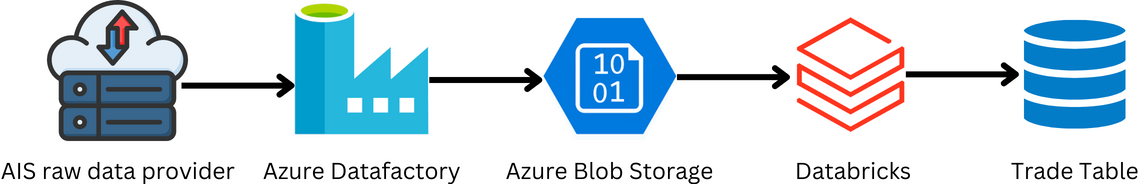
\includegraphics{images/ais_processing.png}
    \caption{AIS Raw Data Processing}
    \label{ais_processing}
\end{figure}

\subsection{Processing Raw AIS data to Trade Flow}

Astrup fearnley receives raw AIS data from external vendor called Exact Earth.
For this there is a pipeline setup on Azure Data Factory which updates raw data every hour in CSV files.

Using databricks following informations are extracted from the raw data and processed further:

\begin{table}[ht]
    \centering
    \small % reduce font size
    \begin{tabular}{|l|p{0.4\linewidth}|l|}
        \hline
        Column              & Description                                                      & Data Type               \\
        \hline
        IMO                 & International Maritime Organization 2                            & Number                  \\
        \hline
        \text{TS\_POS\_UTC} & Date and Time of Last Position AIS Message in UTC                & YYYYMMDDHHmmSS          \\
        \hline
        POSITION            & WGS84 Point, Geographic Location                                 & Geometry                \\
        \hline
        LONGITUDE           & WGS 84 Longitude Coordinate 2                                    & Number, Decimal Degrees \\
        \hline
        LATITUDE            & WGS 84 Latitude Coordinate                                       & Number, Decimal Degrees \\
        \hline
        SOG                 & Speed over Ground                                                & Number, Knots           \\
        \hline
        HEADING             & Heading                                                          & Number, Degrees         \\
        \hline
        \text{NAV\_STATUS}  & Navigational Status                                              & Text                    \\
        \hline
        DESTINATION         & Port of Destination                                              & Text                    \\
        \hline
        ETA                 & Month, Day, Hour, and Minute of Estimated Time of Arrival in UTC & MMDDHHmm                \\
        \hline
        DRAUGHT             & Vessel Draught                                                   & Number, Metres          \\
        \hline
    \end{tabular}
    \caption{Important data from raw AIS data}
    \label{tab:ais_raw_data}
\end{table}

\subsubsection{Shipstops}

To detect a ship stop, the speed is estimated by calculating the distance and time interval between the current and previous AIS signal:

\begin{equation}
    \Delta d = \text{geodesic distance between latlong-coordinates in the current and previous signals.}
\end{equation}

\begin{equation}
    \Delta t = t_2 - t_1, \text{where } t_2 \text{ and } t_1 \text{ are the current and previous timestamps respectively.}
\end{equation}

\begin{equation}
    v = \frac{\Delta t}{\Delta d}, \text{estimated velocity in knots.}
\end{equation}

If the estimated velocity is higher than 30 knots, the row is filtered out from the table because none of the ships can reach this velocity. A shipstop is defined as having a reported speed or estimated speed less than 3 knots, and the tmp\_shipstopped0 table is created with these rows.

To distinguish between arrivals and departures, two shipstopped-tables are created:

Shipstopped: tmp\_shipstopped0 is joined with itself on latlong1-coordinates and \newline RowID = RowID - 1.
This gives the current and previous observation of the ship inside a latlong-square with the same one-decimal coordinates.
This table (b) is again left-joined with tmp\_shipstopped0 and filtered on b.RowID is null. So we are left with the rows where the ship changes latlong1-coordinates in each observation.

Shipstopped2 (Departures): Same as Shipstopped but tmp\_shipstopped0 is joined with itself on latlong1-coordinates and RowID = RowID + 1.


The following figure will be used from here: Ekaterina (IMO: 9196644) trade between Fujairah and Zhanjiang.

\begin{figure}[h]
    \centering
    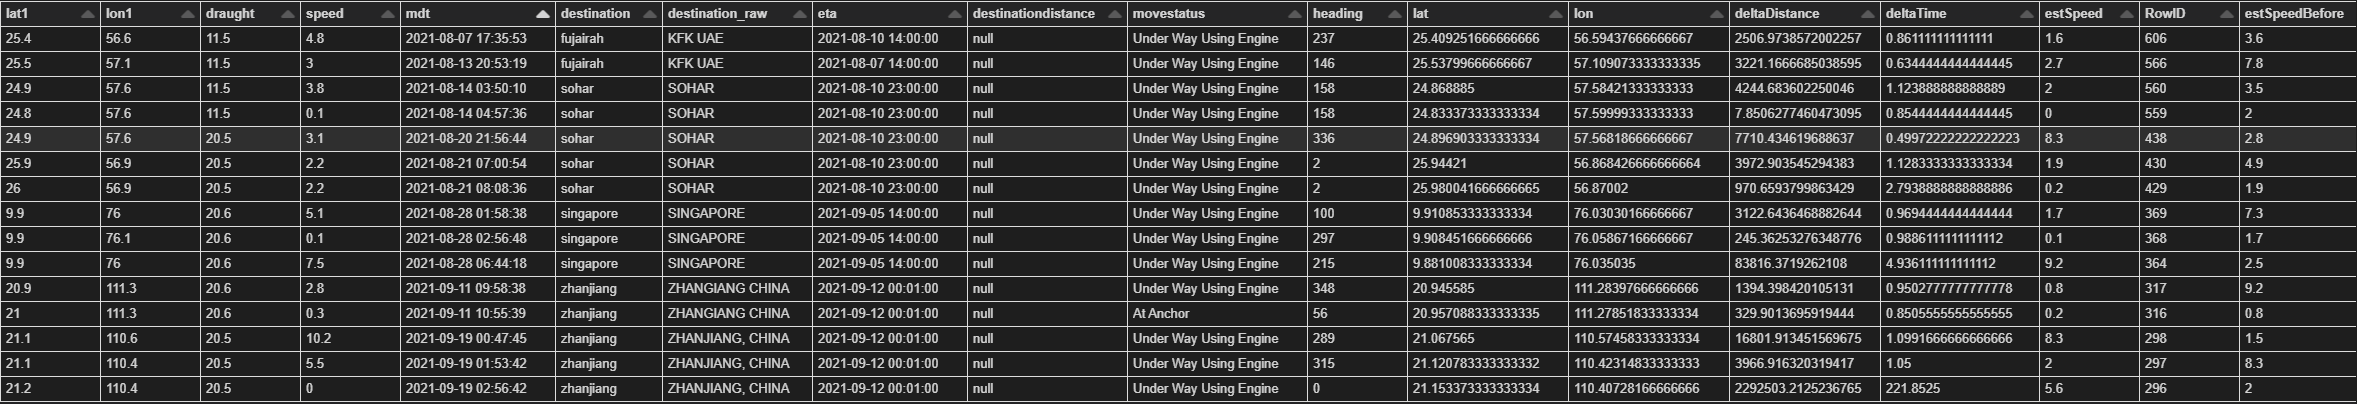
\includegraphics[width=1\textwidth]{images/ship_stop1.png}
    \caption{Shipstopped(Arrivals) for Ekaterina (IMO: 9196644)}
    \label{ship_stop1}
\end{figure}

\begin{figure}[h]
    \centering
    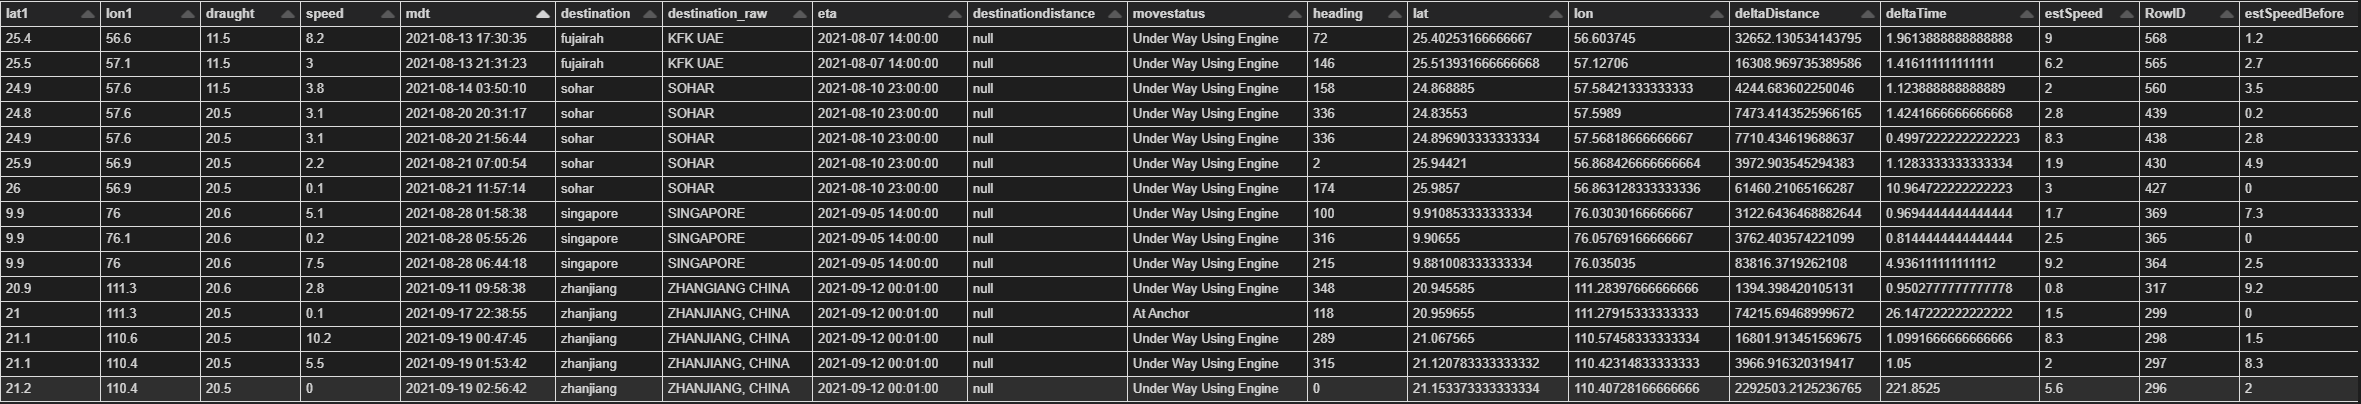
\includegraphics[width=1\textwidth]{images/ship_stop2.png}
    \caption{Shipstopped2(Departures) Ship Stops for Ekaterina (IMO: 9196644)}
    \label{ship_stop2}
\end{figure}

\subsubsection{Ship Callport}

To determine whether the arrival and/or departure observations are part of a port stop, we follow these steps:

1. Left Join with LatLongPort3 Table:
The \textbf{LatLongPort3} table is left-joined with the union of the ShipStopped tables.
This results in a new table containing all the arrival and departure measurements along with their corresponding destination names based on the latlong-position.

2. Obtain ShipCallPort Table:
The \textbf{ShipCallPort} table is obtained by lagging the MDT (Mean Draft) and draught columns.
This process allows us to retrieve the timestamps and draught values before and after the port stop.

3. Filter Stops Less Than 3 Hours:
Finally, we filter out the stops that have a duration of less than 3 hours, as they are likely not significant port stops.

Overall, this approach helps us identify and analyze port stops in the data, enabling further insights into ship movements and activities in specific ports.

\begin{figure}[h]
    \centering
    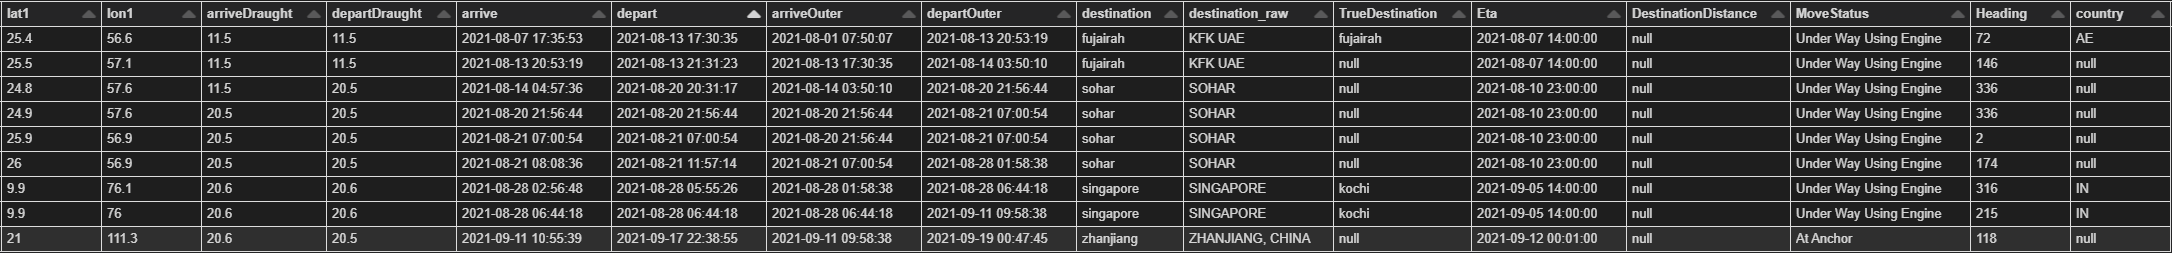
\includegraphics[width=1\textwidth]{images/ship_callport.png}
    \caption{ship callport}
    \label{ship_callport}
\end{figure}

\subsubsection{Ship Travel}

The \textbf{Shiptravel} table is created from the \textbf{Shiptravel\_} table left-joined with the \textbf{ShipCallPort} table on arrival timestamp per IMO-number. This process provides an overview of the total travel route and the ports where the ship called. The destination name, country, and arrival timestamp are concatenated into an array column called \textbf{TrueDestinationArray}.

Subsequently, the \textbf{ShipTravelTrue} table is created by selecting the last value of \textbf{TrueDestinationArray} per IMO-number. This table offers a concise representation of the ship's true travel destinations.

From the \textbf{ShipTravelTrue} table, the \textbf{export-table} is derived by selecting the last portstop and concatenating the destination name and MDT (Mean Draft) to create the \textbf{leg-column}. This results in a table that presents the final destination and the MDT value for the ship's last port stop, providing valuable insights into the ship's final leg of the journey.

\begin{figure}[h]
    \centering
    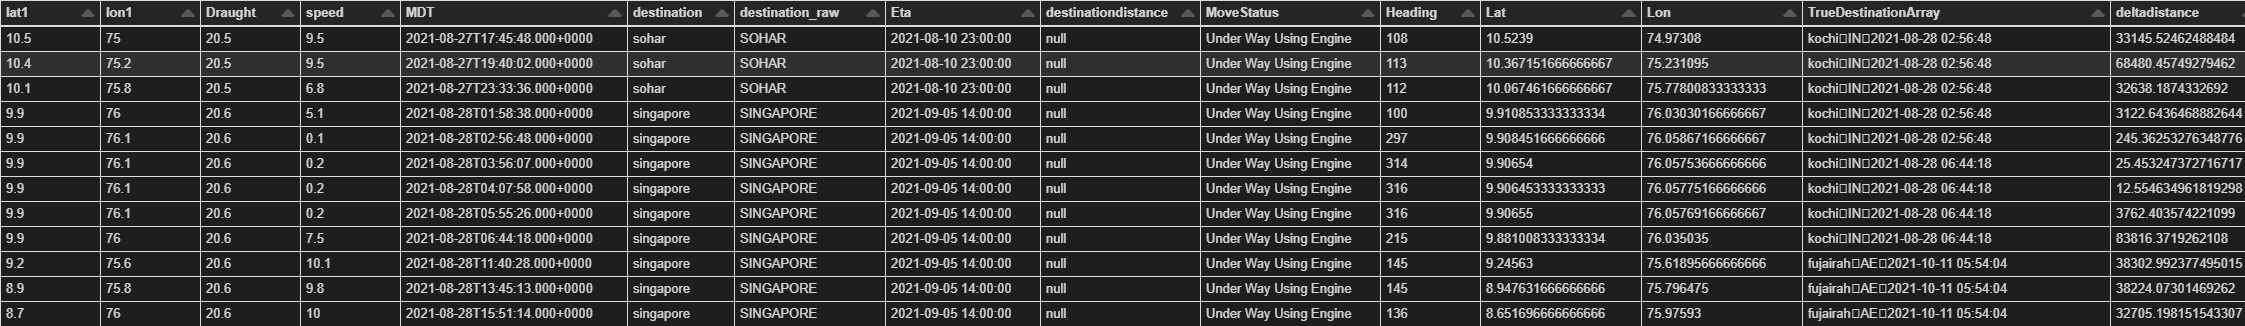
\includegraphics[width=1\textwidth]{images/ship_travel.png}
    \caption{shiptraveltrue Table}
    \label{ship_travel}
\end{figure}

From Figure \ref{ship_travel}, we can observe that the destination-column is not necessarily the same as the TrueDestinationArray.

\subsubsection{Trade Table}

\textbf{Tradetable13Bx} is derived from ShipTravel through several steps of data processing and \newline calculations.
Initially, \textbf{Tradetabletmp} is obtained by estimating the speed and deltaDistance between observations in \textbf{ShipTravelTrue},
filtering out rows with estimated speed above 30 knots, and extracting TrueDestinationArray components.
\textbf{Tradetable0} is defined at the arrival timestamp and unioned with \textbf{tmp\_etatradetableadditions} to create Tradetable.
The \textbf{tmp\_etatradetableadditions} table is created by examining ETA and nextETA values in \newline \textbf{Tradetabletmp} and setting flag values accordingly.

Next, \textbf{Tradetable\_C} is derived by adjusting the distanceTravelledNm-column using row numbers for each IMO and TrueDestination to identify trips to specific destinations.
\newline \textbf{Tradetable\_collapsed} is then created by left joining the \textbf{ShipCallPort} table with \newline  \textbf{Tradetable\_C} and adjusting columns based on individual trip logic.

Further processing is done in \textbf{Tmp\_tradetable0}, including lagging columns and left joining with \textbf{ShiftDraughtChange} table.
\textbf{Tmp\_tradetable1} adds additional rows to \textbf{tmp\_details} table.
Finally, \textbf{Tradetable13x} is derived by modifying columns based on certain thresholds and rules, and
\textbf{Tradetable13Bx} is obtained by aggregating information from \textbf{Tradetable13x} and calculating sumLegDistance and HoursTravelled\_.

In summary, \textbf{Tradetable13Bx} is obtained through a series of data manipulations and calculations starting from ShipTravel.

\begin{figure}[h]
    \centering
    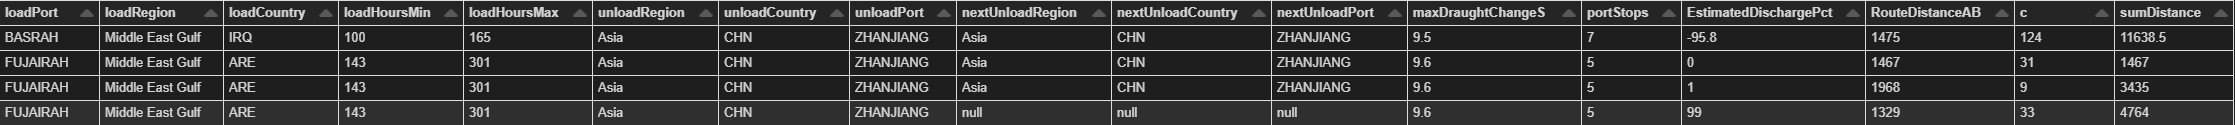
\includegraphics[width=1\textwidth]{images/tradetable13bx.png}
    \caption{Tradetable13Bx}
    \label{tradetable13bx}
\end{figure}